% File encoding
\usepackage[utf8]{inputenc}

% Languages
\usepackage[main=english]{babel} %,[ngerman]

% classicthesis setup
\PassOptionsToPackage{%
  %drafting,%
  dottedtoc,%
  eulerchapternumbers,
  %listings,%
  %parts,%
  floatperchapter, pdfspacing,%
  beramono,%
  %minionprospacing,
  %subfig,%
  %eulermath,%
  a5paper,%
}{classicthesis}

%
% Document information
%
\newcommand{\myTitle}{%
  Sequence alignment using A*\xspace%
}
\newcommand{\myPlainTitle}{%
  Sequence alignment using A*\xspace%
}

\newcommand{\myDissNumber}{?}
\newcommand{\myName}{Pesho Ivanov\xspace}
\newcommand{\myUni}{\protect{ETH Z\"urich}\xspace}
\newcommand{\myLocation}{Z\"urich\xspace}
\newcommand{\myTime}{2022\xspace}

% DOI
\newcommand{\myDOI}{10.3929/ethz-a-}

% Work version info
\newcommand{\worktodo}[1]{\textcolor{red}{\textbf{TODO}: #1}}
\usepackage{scrtime}
\newcommand{\workdraft}{\textcolor{gray}{Draft, \today{}---\thistime}}
% \renewcommand{\workdraft}{}
% \renewcommand{\worktodo}{}

\input{preamble/hyphenation}

\newcounter{dummy}
\newlength{\abcd}

\newcommand{\ie}{i.\,e.\xspace}
\newcommand{\Ie}{I.\,e.\xspace}
\newcommand{\eg}{e.\,g.\xspace}
\newcommand{\Eg}{E.\,g.\xspace}

\usepackage{csquotes}  % smart quotes
\usepackage[T1]{fontenc}
\usepackage{xspace}
\usepackage{textcomp}
\usepackage{mparhack}
\usepackage{relsize}

% Biblatex
\usepackage[
  style=nature,%
  %style=science, article-title=true,%
  natbib=true,%
  clearlang=true,%
  backend=bibtex,%
]{biblatex}

\ExecuteBibliographyOptions{%
  %--- Backend --- --- ---
  bibwarn=true, %
  bibencoding=auto, % (ascii, inputenc, <encoding>)
  %--- Sorting --- --- ---
  sorting=none, % Sort by name, title, year.
  % other options: 
  % nty        Sort by name, title, year.
  % nyt        Sort by name, year, title.
  % nyvt       Sort by name, year, volume, title.
  % anyt       Sort by alphabetic label, name, year, title.
  % anyvt      Sort by alphabetic label, name, year, volume, title.
  % ynt        Sort by year, name, title.
  % ydnt       Sort by year (descending), name, title.
  % none       Do not sort at all. All entries are processed in citation order.
  % debug      Sort by entry key. This is intended for debugging only.
  %
  sortcase=true,
  sortlos=los, % (bib, los) The sorting order of the list of shorthands
  sortcites=true, % do/do not sort citations according to bib	
  %--- Dates --- --- ---
  date=comp,  % (short, long, terse, comp, iso8601)
  %	origdate=
  %	eventdate=
  %	urldate=
  %	alldates=
  datezeros=true, %
  dateabbrev=true, %
  %--- General Options --- --- ---
  maxnames=3,
  minnames=1,
  maxbibnames=100, % do not abbreviate names in bibliography
  %	autocite= % (plain, inline, footnote, superscript) 
  autopunct=true,
  language=auto,
  babel=none, % (none, hyphen, other, other*)
  block=none, % (none, space, par, nbpar, ragged)
  notetype=foot+end, % (foot+end, footonly, endonly)
  hyperref=true, % (true, false, auto)
  backref=false,
  backrefstyle=three, % (none, three, two, two+, three+, all+)
  backrefsetstyle=setonly, %
  indexing=false, % 
  % options:
  % true       Enable indexing globally.
  % false      Disable indexing globally.
  % cite       Enable indexing in citations only.
  % bib        Enable indexing in the bibliography only.
  refsection=none, % (part, chapter, section, subsection)
  refsegment=none, % (none, part, chapter, section, subsection)
  abbreviate=true, % (true, false)
  defernumbers=false, % 
  punctfont=false, % 
  arxiv=abs, % (ps, pdf, format)	
  %--- Style Options --- --- ---	
  % The following options are provided by the standard styles
  isbn=false,%
  url=false,%
  doi=false,%
  eprint=false,%	
}%	

% Suppress all date fields except the year
\AtEveryBibitem{%
  \clearfield{day}%
  \clearfield{month}%
  \clearfield{endday}%
  \clearfield{endmonth}%
}

\DeclareRedundantLanguages{en,EN,English}{english}

% Use only the first page number in a given range
\DeclareFieldFormat{pages}{\mkfirstpage{#1}}

\let\origcite\cite%
\def\cite#1{\unskip~\origcite{#1}}

% Math stuff
\usepackage{amsmath}
\usepackage{mathtools}
\usepackage{isomath}

% Figures, tables, and captions
\usepackage{tabularx}
\usepackage{ltablex}
\setlength{\extrarowheight}{3pt}
\newcommand{\tableheadline}[1]{\multicolumn{1}{c}{\spacedlowsmallcaps{#1}}}
\newcommand{\myfloatalign}{\centering}
\usepackage{floatrow}
\usepackage{caption}
\captionsetup{format=hang,font=small,labelfont={sc},margin=5pt}
\usepackage{subcaption}
\captionsetup[sub]{margin=0pt,font=small,labelfont={rm}}

\usepackage{blindtext}

\usepackage[dvipsnames]{xcolor}
\usepackage[%
  hyperfootnotes=false,%
  pdfpagelabels,%
  % pdfa,%
]{hyperref}
\usepackage{hyperxmp}
%\pdfcompresslevel=9
%\pdfadjustspacing=1
\hypersetup{%
  %pdfstartpage=3, pdfstartview=FitV,%
  % following line: colored links (web version)
  colorlinks=true, linktocpage=true,%
  % following line: all links in black (for printing)
  %colorlinks=false, linktocpage=false, pdfborder={0 0 0},%
  breaklinks=true, pdfpagemode=UseNone, pageanchor=true, pdfpagemode=UseOutlines,%
  plainpages=false, bookmarksnumbered, bookmarksopen=true, bookmarksopenlevel=1,%
  hypertexnames=true, pdfhighlight=/O,%nesting=true,%frenchlinks,%
  pdftitle={\myPlainTitle},%
  pdfauthor={\myName},%
  pdfcopyright={Copyright (C) \myTime, \myName},%
  pdfsubject={},%
  pdfkeywords={},%
  pdflang={en},%
}

% Graphics
\usepackage{graphicx}
\usepackage{rotating}
\usepackage{tikz}
\usepackage{pgfplots}
\pgfplotsset{compat=newest}
\usetikzlibrary{shapes.geometric}

\newcommand*\circled[1]{
  \tikz[baseline=(char.base)]{
     \node[shape=circle,draw,inner sep=1pt,font=\footnotesize] (char) {#1};}}

\renewcommand*{\figureautorefname}{Figure}
\renewcommand*{\tableautorefname}{Table}
\renewcommand*{\partautorefname}{Part}
\renewcommand*{\chapterautorefname}{Chapter}
\renewcommand*{\sectionautorefname}{Section}
\renewcommand*{\subsectionautorefname}{Section}
\renewcommand*{\subsubsectionautorefname}{Section}
\providecommand{\subfigureautorefname}{\figureautorefname}%
\usepackage[capitalize]{cleveref}

\PassOptionsToPackage{printonlyused}{acronym}
\usepackage{acronym}

\usepackage{enumitem}

\usepackage{scrhack}
\usepackage{classicthesis}

\KOMAoptions{headinclude=true,footinclude=false}
\setlength{\textwidth}{11.6cm} % 10 pt font
\areaset[current]{\textwidth}{1.618034\textwidth}

% Page numbers in plain style (chapter titles)
\clearscrplain
\ofoot[\pagemark]{}
% Adjust distance to footer (default is too large)
\setlength{\footskip}{19pt}

\definecolor{chapter-color}{cmyk}{1, 0.50, 0, 0.25}
\definecolor{link-color}{cmyk}{1, 0.50, 0, 0.25}
\definecolor{cite-color}{cmyk}{0, 0.7, 0.9, 0.2}

% Hyperref
\usepackage{bookmark}
\hypersetup{
  %urlcolor=webbrown, linkcolor=RoyalBlue, citecolor=webgreen, %pagecolor=RoyalBlue,%
  %urlcolor=webbrown, linkcolor=Maroon, citecolor=webgreen,%
  %urlcolor=link-color, linkcolor=link-color, citecolor=cite-color,%
  urlcolor=Black, linkcolor=Black, citecolor=Black, %pagecolor=Black,%
}

% Chapter font
\let\chapterNumber\undefined%
\newfont{\chapterNumber}{eurb10 scaled 5500}

\usepackage{siunitx}
\sisetup{
  separate-uncertainty,
  repeatunits=false,
  detect-family,
  unit-mode=text,
}
\DeclareSIUnit\au{a.u.}
\let\u=\SI%

\newcommand{\productcode}[1]{\figureversion{lining}#1}

% TOC
\renewcommand{\cftpartfont}{\color{chapter-color}\normalfont}%
\renewcommand{\cftpartpagefont}{\normalfont}%

% Chapter number on inside
\titleformat{\chapter}[display]%
  {\relax}{\vspace*{-3\baselineskip}\makebox[\linewidth][r]{\color{halfgray}\chapterNumber\thechapter}}{10pt}%
  {\raggedright\spacedallcaps}[\normalsize\vspace*{.8\baselineskip}\titlerule]%

% Chapter abstract
\def\chapterabstract#1{%
  \begingroup
  \baselineskip1.3em
  \leftskip1em
  \rightskip\leftskip\itshape#1
  \par
  \endgroup
}

% Chapter quotes
% Adapted from: <http://tex.stackexchange.com/questions/53377/inspirational-quote-at-start-of-chapter>
\setkomafont{dictumtext}{\itshape\small}%
\setkomafont{dictumauthor}{\normalfont}
\renewcommand*{\dictumwidth}{0.6\textwidth}
\renewcommand*{\dictumrule}{}
\renewcommand*\dictumauthorformat[1]{--- #1}

% Subfigure labels (manual)
\newcommand{\subfig}[1]{(#1)}

% CV
\newcommand{\cvleft}[1]{\begin{minipage}[t]{2.5cm}\begin{flushright}#1\end{flushright}\end{minipage}\hspace{5mm}}
\newcommand{\cvright}[1]{\begin{minipage}[t]{8cm}{#1}\end{minipage}}

% Footnote without number
\newcommand\blfootnote[1]{%
  \begingroup
  \renewcommand\thefootnote{}\footnote{#1}%
  \addtocounter{footnote}{-1}%
  \endgroup
}

% Put pages on A4 w/ crop marks
%\usepackage[a4,center,cam]{crop}

% Widow and club penalties
\clubpenalty = 10000
\widowpenalty = 10000
%\displaywidowpenalty = 10000

\renewcommand{\sfdefault}{phv}

\usepackage{amsmath}
\usepackage{amssymb}
\usepackage{amsthm}

\usepackage{latexsym}  % \leadsto

\usepackage{booktabs}   % tables: toprule, midrule
\usepackage{colortbl}
\usepackage{dsfont} % beautiful 1
\usepackage{float}
\usepackage{ragged2e}

\usepackage[]{todonotes}  % [disable]
\usepackage{mathtools}   % smashoperator 

\usepackage{graphicx}
\usepackage{epigraph}

\usepackage{svg}
\usepackage{tikz}
\usetikzlibrary{tikzmark,decorations.pathreplacing,calc}

\usepackage{multirow}   % tables

\usepackage{numprint}   % tables
\npdecimalsign{.}

\setcounter{tocdepth}{3}

\usepackage{thmtools}
\usepackage{thm-restate}
\usepackage{etoolbox}
\declaretheorem[name=Theorem]{thm}
%\declaretheorem[name=Proposition]{prop}
\declaretheorem[name=Lemma]{lem}
\declaretheorem[name=Definition]{definition}
%\declaretheorem[name=Observation]{observation}
\declaretheorem[name=Corollary]{cor}
\declaretheorem[name=Remark]{remark}

\crefname{thm}{theorem}{theorems}
\Crefname{thm}{Theorem}{Theorems}
\crefname{lem}{lemma}{lemmas}
\Crefname{lem}{Lemma}{Lemmas}
\crefname{cor}{corollary}{corollaries}
\Crefname{cor}{Corollary}{Corollaries}
\crefname{remark}{remark}{remarks}
\Crefname{remark}{Remark}{Remarks}

\newcommand{\A}[0]{A$^\star$\xspace}
\newcommand{\csh}[0]{chaining seed heuristic\xspace}
\newcommand{\Csh}[0]{Chaining seed heuristic\xspace}
\newcommand{\CSH}[0]{CSH\xspace}
\newcommand{\sh}[0]{seed heuristic\xspace}
\newcommand{\Sh}[0]{Seed heuristic\xspace}
\newcommand{\SH}[0]{SH\xspace}

\newcommand{\lcs}[0]{\mbox{LCS}\xspace}
\newcommand{\lcskpp}[0]{\mbox{LCSk++}\xspace}
\newcommand{\pa}[0]{pairwise alignment\xspace}
\newcommand{\ed}[0]{\mbox{ed}\xspace}

% tool names
\newcommand{\difftool}[0]{\mbox{\textsc{diff}}\xspace}
\newcommand{\edlib}[0]{\mbox{\textsc{Edlib}}\xspace}
\newcommand{\oldwfa}[0]{\mbox{\textsc{WFA}}\xspace}
\newcommand{\wfa}[0]{\mbox{\textsc{BiWFA}}\xspace}
\newcommand{\seqan}[0]{\mbox{\textsc{SeqAn}}\xspace}
\newcommand{\parasail}[0]{\mbox{\textsc{Parasail}}\xspace}
\newcommand{\astarpa}[0]{\mbox{\textsc{A*PA}}\xspace}
\newcommand{\astarix}[0]{\mbox{\textsc{AStarix}}\xspace}
\newcommand{\dijkstra}[0]{\mbox{Dijkstra}\xspace}

\patchcmd{\paragraph}{\itshape}{\bfseries\boldmath}{}{}

\setlength{\abovecaptionskip}{5pt plus 0pt minus 0pt}

\newcommand{\Oh}[0]{O}

\newcommand{\seeds}{\mathcal S}
\newcommand{\matches}{\mathcal M}

% Commands for A* functions
\newcommand{\st}[2]{\langle #1, #2 \rangle}
\newcommand{\g}{g^*\!}
\newcommand{\h}{h^*\!}
\newcommand{\ssh}{_{\mathrm{sh}}}
\newcommand{\scsh}{_{\mathrm{csh}}}
\newcommand{\hsh}{h\ssh\!}
\newcommand{\hcsh}{h\scsh\!}
\newcommand{\hshM}{h\ssh^\matches\!}
\newcommand{\hcshM}{h\scsh^\matches\!}
\newcommand{\hh}{\hat h}
\newcommand{\hshS}{\hat h\ssh\!}
\newcommand{\hcshS}{\hat h\scsh\!}
\newcommand{\Path}{\pi^*}

\newcommand{\Pot}{P}
\newcommand{\spot}{r}
\newcommand{\cost}{\operatorname{cost}}
\newcommand{\matchscore}{\operatorname{score}}
\newcommand{\seedscore}{\operatorname{score}}
\newcommand{\statescore}{S}
\newcommand{\chainscore}{S_{\mathrm{chain}}}
\newcommand{\shscore}{S_{\mathrm{sh}}}
\newcommand{\cshscore}{S_{\mathrm{csh}}}

\newcommand{\layer}{\mathcal L}

\newcommand{\start}{\operatorname{start}}

\newcommand{\substr}[3]{#1_{#2{\dots}#3}}

\renewcommand{\path}[2]{(#1{\leadsto}#2)}

% Fig.2
\newcommand{\bluecircle}{
\includegraphics[height=4pt]{imgs/fig2-symbols/blue-circle.pdf}}
\newcommand{\greencircle}{
\includegraphics[height=4pt]{imgs/fig2-symbols/green-circle.pdf}}
\newcommand{\cross}{
\includegraphics[height=4pt]{imgs/fig2-symbols/cross.pdf}}
\newcommand{\seed}{
\includegraphics[width=6pt]{imgs/fig2-symbols/seed.pdf}}
\newcommand{\match}{
\includegraphics[height=4pt]{imgs/fig2-symbols/match.pdf}}
\newcommand{\redcolumn}{
\includegraphics[height=5pt]{imgs/fig2-symbols/red-column.pdf}}
\newcommand{\greencolumn}{
\includegraphics[height=5pt]{imgs/fig2-symbols/green-column.pdf}}

% Fig.3
\newcommand{\bluesquare}{
\includegraphics[height=4pt]{imgs/fig3-symbols/bluesquare.pdf}}
\newcommand{\greensquare}{
\includegraphics[height=4pt]{imgs/fig3-symbols/greensquare.pdf}}
\newcommand{\blackmatch}{
\includegraphics[height=5pt]{imgs/fig3-symbols/blackmatch.pdf}}
\newcommand{\redmatch}{
\includegraphics[height=5pt]{imgs/fig3-symbols/redmatch.pdf}}

% Plots
\newcommand{\edlibsymbol}{
\includegraphics[height=4pt]{imgs/plots-symbols/edlib.pdf}}
\newcommand{\wfasymbol}{
\includegraphics[height=4pt]{imgs/plots-symbols/wfa.pdf}}
\newcommand{\shsymbol}{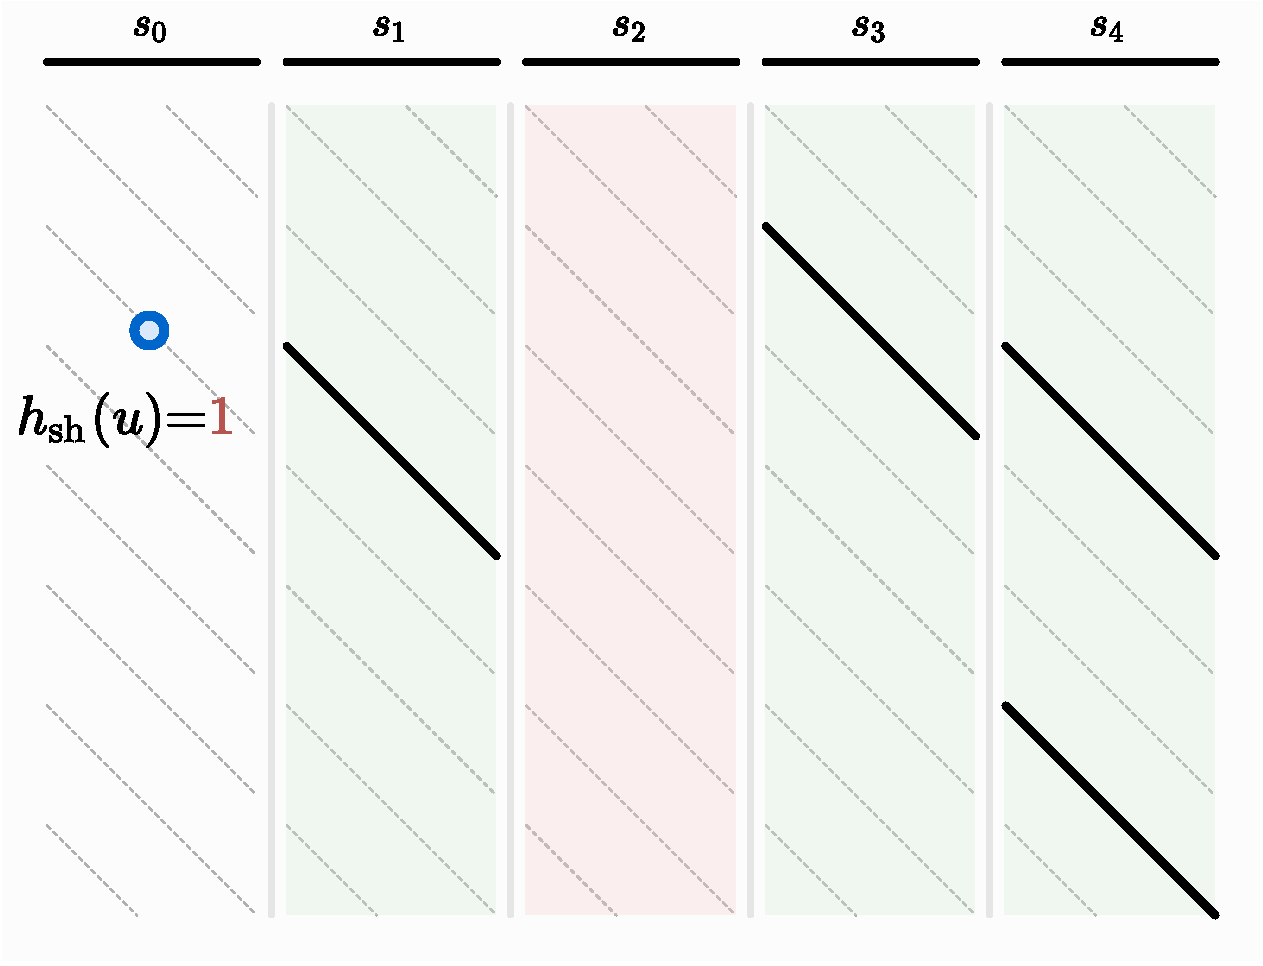
\includegraphics[height=4pt]{imgs/plots-symbols/sh.pdf}}
\newcommand{\shsymbolsq}{
\includegraphics[height=4pt]{imgs/plots-symbols/sh-down.pdf}}
\newcommand{\cshsymbol}{
\includegraphics[height=4pt]{imgs/plots-symbols/csh.pdf}}
\newcommand{\cshsymbolsq}{
\includegraphics[height=4pt]{imgs/plots-symbols/csh-down.pdf}}

% TODO
%\newcommand{\bp}{\unit{\,bp}}
%\newcommand{\kbp}{\unit{\,kbp}}
\newcommand{\bp}{\,bp}
\newcommand{\kbp}{\,kbp}
% TODO: remove \qty and \unit in favor of siunitx
\newcommand{\qty}[2]{#1\ #2}
\newcommand{\unit}[1]{#1} 

% datasets
\newcommand{\datasetOne}{CHM13}
\newcommand{\datasetTwo}{NA12878}

% paper-trie

\usepackage{graphicx}     % Used for displaying a sample figure. If possible,figure files should be included in EPS format.

\usepackage{wrapfig}
\usepackage[T1]{fontenc}  %% for small caps \textsc
\usepackage{libertine}
\usepackage{xspace}
\usepackage{amsmath}
\usepackage{amssymb}
\usepackage{amsfonts}
\usepackage{booktabs}
\newcommand{\ra}[1]{\renewcommand{\arraystretch}{#1}}

\usepackage{multirow}
\usepackage{xr}  % for importing external .aux (for the appendix)
\usepackage{filecontents}  % for embedding the .aux into .tex

\usepackage{numprint}
\npdecimalsign{.}

% add qed to all proofs
%\let\oldProof\proof
%\let\oldEndProof\endproof
%\renewenvironment{proof}
%{\oldProof}
%{\qed \oldEndProof}

\usepackage{subcaption}  % for subfigures 
\captionsetup{compatibility=false}  % a workaround for "The `subcaption' package does not work correctly in compatibility mode."

%%%%%%%%%%%%%%%%%%%%%%%%%
% ALGORITHM DEFINITIONS %
%%%%%%%%%%%%%%%%%%%%%%%%%
\usepackage{algorithm}
\usepackage[noend]{algpseudocode}  % layout for algorithmicx
\algdef{SE}[SUBALG]{Indent}{EndIndent}{}{\algorithmicend\ }%
\algtext*{Indent}
\algtext*{EndIndent}

\usepackage{fontawesome}
\usepackage[clock]{ifsym}  % special symbols

% temporary (for debugging)
\usepackage[]{todonotes}  % [disable]

\usepackage{standalone}

% Description: This file enables using \cref to references Figures, Sections,
% Equations, etc.
%
% Usage: % Description: This file enables using \cref to references Figures, Sections,
% Equations, etc.
%
% Usage: % Description: This file enables using \cref to references Figures, Sections,
% Equations, etc.
%
% Usage: \input{headers/lqa/references}

%%%%%%%%%%%%%%
% REFERENCES %
%%%%%%%%%%%%%%

% Package documentation:
% http://ftp.math.purdue.edu/mirrors/ctan.org/macros/latex/contrib/cleveref/cleveref.pdf

% PACKAGE OPTIONS:
%
% capitalize: always capitalize cross-reference names, regardless of where they
% appear in the sentence, writing Theorem 1 and Equation 3 (as opposed to
% theorem 1 and equation 3)
%
% noabbrev:  avoid abbreviations (\eg use Figure instead of Fig.). Note: To
% avoid all abbreviations, you must also check all manually defined reference
% names in this file.

%\usepackage[capitalize]{cleveref}

% required for proper hyperrefs into algorithm lines
% use "renewcommand" instead of "newcommand" if \eg the document class already defines this
\makeatletter
\newcommand\theHALG@line{\thealgorithm.\arabic{ALG@line}}
\makeatother

% OVERRIDE CREF FORMAT:
%
% Override the cref format, \eg, for sections to: §1.2
%
% #1: formatted version of the label counter
%
% #2, #3: beginning and end of the part of the cross-reference that forms the
% hyperlink
%
% Example: Override the cref format for equations to, \eg, Eq.~(1)
%
% \crefformat{equation}{Eq.~(#2#1#3)}

\crefformat{section}{\S#2#1#3}

% referencing sections without labels (\eg, from citations)
\newcommand{\secref}[1]{\S#1}

% OVERRIDE CREF FORMAT FOR RANGES:
%
% override the cref format for ranges of sections, \eg: §1.2 to §1.3
%
% #1, #2: formatted versions of the two label counters defining the reference
% range
%
% #3, #4: denote the beginning and end of the hyperlink for the first reference
%
% #5, #6: denote the beginning and end of the hyperlink for the second reference
\crefrangeformat{section}{\S#3#1#4\crefrangeconjunction\S#5#2#6}

% OVERRIDE CREF FORMAT FOR LISTS:
%
% override the cref format for multiple sections, \eg,:
%
% Argument 1: the cross-reference type
%
% Argument 2: the format for the first cross-reference in a list
%
% Argument 3: the format for the second cross-reference in a list of two
%
% Argument 4: the format for the middle cross-references in a list of more than two
%
% Argument 5: the format for the last cross-reference in a list of more than two
\crefmultiformat{section}{\S#2#1#3}{\crefpairconjunction\S#2#1#3}{\crefmiddleconjunction\S#2#1#3}{\creflastconjunction\S#2#1#3}

% ADAPT CONJUNCTION
%
% Adapt the conjunction used in a reference range, to, \eg: Figs. 1-2
\newcommand{\crefrangeconjunction}{--}

% CUSTOMIZE/ADD REFERENCE NAME
%
% Customize the cross-reference name for a given cross-reference type
%
% Argument 1: the cross-reference type
% 
% Argument 2: singular form of name
%
% Argument 3: plural form of name
% 
% Examples:
% 
% \crefname{section}{Sec.}{Sections}
\crefname{theorem}{Thm.}{Thms.}
\crefname{thm}{Thm.}{Thms.}
% \crefname{lem}{Lem.}{Lemmas}
% \crefname{lstlisting}{Listing}{listings}
% \crefname{algorithm}{Alg.}{Algs.}
% \crefname{example}{Ex.}{Exs.}
% \crefname{table}{Tab.}{Tabs.}
\crefname{listing}{Lst.}{listings}
\crefname{line}{Lin.}{Lin.}
\crefname{appendix}{App.}{App.}

% references without labels (\eg, from citations)
% \newcommand{\thmref}[1]{Thm.~#1}
% \newcommand{\lemref}[1]{Lem.~#1}
% \newcommand{\appref}[1]{App.~#1}
% \newcommand{\algoref}[1]{Alg.~#1}
% \newcommand{\exref}[1]{Ex.~#1}
% \newcommand{\tabref}[1]{Tab.~#1}
% \newcommand{\propref}[1]{Prop.~#1}
% \newcommand{\figref}[1]{Fig.~#1}

%%%%%%%%%%%%
% APPENDIX %
%%%%%%%%%%%%

\newcommand{\appref}[1]{%
	\ifbool{includeappendix}{\cref{SEED#1}}{the appendix}%
}
\newcommand{\Appref}[1]{%
	\ifbool{includeappendix}{\cref{SEED#1}}{The appendix}%
}

%%%%%%%%%%%%%%%%%%%%%%%%%%%
% OPTIONAL CUSTOMIZATIONS %
%%%%%%%%%%%%%%%%%%%%%%%%%%%

% Alias a counter to a different cross-reference type.
%
% Example: Write Fig.~5 for \cref{SEEDsec:abc}
%
% \crefalias{section}{figure}


%%%%%%%%%%%%%%
% REFERENCES %
%%%%%%%%%%%%%%

% Package documentation:
% http://ftp.math.purdue.edu/mirrors/ctan.org/macros/latex/contrib/cleveref/cleveref.pdf

% PACKAGE OPTIONS:
%
% capitalize: always capitalize cross-reference names, regardless of where they
% appear in the sentence, writing Theorem 1 and Equation 3 (as opposed to
% theorem 1 and equation 3)
%
% noabbrev:  avoid abbreviations (\eg use Figure instead of Fig.). Note: To
% avoid all abbreviations, you must also check all manually defined reference
% names in this file.

%\usepackage[capitalize]{cleveref}

% required for proper hyperrefs into algorithm lines
% use "renewcommand" instead of "newcommand" if \eg the document class already defines this
\makeatletter
\newcommand\theHALG@line{\thealgorithm.\arabic{ALG@line}}
\makeatother

% OVERRIDE CREF FORMAT:
%
% Override the cref format, \eg, for sections to: §1.2
%
% #1: formatted version of the label counter
%
% #2, #3: beginning and end of the part of the cross-reference that forms the
% hyperlink
%
% Example: Override the cref format for equations to, \eg, Eq.~(1)
%
% \crefformat{equation}{Eq.~(#2#1#3)}

\crefformat{section}{\S#2#1#3}

% referencing sections without labels (\eg, from citations)
\newcommand{\secref}[1]{\S#1}

% OVERRIDE CREF FORMAT FOR RANGES:
%
% override the cref format for ranges of sections, \eg: §1.2 to §1.3
%
% #1, #2: formatted versions of the two label counters defining the reference
% range
%
% #3, #4: denote the beginning and end of the hyperlink for the first reference
%
% #5, #6: denote the beginning and end of the hyperlink for the second reference
\crefrangeformat{section}{\S#3#1#4\crefrangeconjunction\S#5#2#6}

% OVERRIDE CREF FORMAT FOR LISTS:
%
% override the cref format for multiple sections, \eg,:
%
% Argument 1: the cross-reference type
%
% Argument 2: the format for the first cross-reference in a list
%
% Argument 3: the format for the second cross-reference in a list of two
%
% Argument 4: the format for the middle cross-references in a list of more than two
%
% Argument 5: the format for the last cross-reference in a list of more than two
\crefmultiformat{section}{\S#2#1#3}{\crefpairconjunction\S#2#1#3}{\crefmiddleconjunction\S#2#1#3}{\creflastconjunction\S#2#1#3}

% ADAPT CONJUNCTION
%
% Adapt the conjunction used in a reference range, to, \eg: Figs. 1-2
\newcommand{\crefrangeconjunction}{--}

% CUSTOMIZE/ADD REFERENCE NAME
%
% Customize the cross-reference name for a given cross-reference type
%
% Argument 1: the cross-reference type
% 
% Argument 2: singular form of name
%
% Argument 3: plural form of name
% 
% Examples:
% 
% \crefname{section}{Sec.}{Sections}
\crefname{theorem}{Thm.}{Thms.}
\crefname{thm}{Thm.}{Thms.}
% \crefname{lem}{Lem.}{Lemmas}
% \crefname{lstlisting}{Listing}{listings}
% \crefname{algorithm}{Alg.}{Algs.}
% \crefname{example}{Ex.}{Exs.}
% \crefname{table}{Tab.}{Tabs.}
\crefname{listing}{Lst.}{listings}
\crefname{line}{Lin.}{Lin.}
\crefname{appendix}{App.}{App.}

% references without labels (\eg, from citations)
% \newcommand{\thmref}[1]{Thm.~#1}
% \newcommand{\lemref}[1]{Lem.~#1}
% \newcommand{\appref}[1]{App.~#1}
% \newcommand{\algoref}[1]{Alg.~#1}
% \newcommand{\exref}[1]{Ex.~#1}
% \newcommand{\tabref}[1]{Tab.~#1}
% \newcommand{\propref}[1]{Prop.~#1}
% \newcommand{\figref}[1]{Fig.~#1}

%%%%%%%%%%%%
% APPENDIX %
%%%%%%%%%%%%

\newcommand{\appref}[1]{%
	\ifbool{includeappendix}{\cref{SEED#1}}{the appendix}%
}
\newcommand{\Appref}[1]{%
	\ifbool{includeappendix}{\cref{SEED#1}}{The appendix}%
}

%%%%%%%%%%%%%%%%%%%%%%%%%%%
% OPTIONAL CUSTOMIZATIONS %
%%%%%%%%%%%%%%%%%%%%%%%%%%%

% Alias a counter to a different cross-reference type.
%
% Example: Write Fig.~5 for \cref{SEEDsec:abc}
%
% \crefalias{section}{figure}


%%%%%%%%%%%%%%
% REFERENCES %
%%%%%%%%%%%%%%

% Package documentation:
% http://ftp.math.purdue.edu/mirrors/ctan.org/macros/latex/contrib/cleveref/cleveref.pdf

% PACKAGE OPTIONS:
%
% capitalize: always capitalize cross-reference names, regardless of where they
% appear in the sentence, writing Theorem 1 and Equation 3 (as opposed to
% theorem 1 and equation 3)
%
% noabbrev:  avoid abbreviations (\eg use Figure instead of Fig.). Note: To
% avoid all abbreviations, you must also check all manually defined reference
% names in this file.

%\usepackage[capitalize]{cleveref}

% OVERRIDE CREF FORMAT:
%
% Override the cref format, \eg, for sections to: §1.2
%
% #1: formatted version of the label counter
%
% #2, #3: beginning and end of the part of the cross-reference that forms the
% hyperlink
%
% Example: Override the cref format for equations to, \eg, Eq.~(1)
%
% \crefformat{equation}{Eq.~(#2#1#3)}

\crefformat{section}{\S#2#1#3}

% OVERRIDE CREF FORMAT FOR RANGES:
%
% override the cref format for ranges of sections, \eg: §1.2 to §1.3
%
% #1, #2: formatted versions of the two label counters defining the reference
% range
%
% #3, #4: denote the beginning and end of the hyperlink for the first reference
%
% #5, #6: denote the beginning and end of the hyperlink for the second reference
\crefrangeformat{section}{\S#3#1#4\crefrangeconjunction\S#5#2#6}

% OVERRIDE CREF FORMAT FOR LISTS:
%
% override the cref format for multiple sections, \eg,:
%
% Argument 1: the cross-reference type
%
% Argument 2: the format for the first cross-reference in a list
%
% Argument 3: the format for the second cross-reference in a list of two
%
% Argument 4: the format for the middle cross-references in a list of more than two
%
% Argument 5: the format for the last cross-reference in a list of more than two
\crefmultiformat{section}{\S#2#1#3}{\crefpairconjunction\S#2#1#3}{\crefmiddleconjunction\S#2#1#3}{\creflastconjunction\S#2#1#3}

% ADAPT CONJUNCTION
%
% Adapt the conjunction used in a reference range, to, \eg: Figs. 1-2
\newcommand{\crefrangeconjunction}{--}

% CUSTOMIZE/ADD REFERENCE NAME
%
% Customize the cross-reference name for a given cross-reference type
%
% Argument 1: the cross-reference type
% 
% Argument 2: singular form of name
%
% Argument 3: plural form of name
% 
% Examples:
% 
% \crefname{section}{Sec.}{Sections}
% \crefname{theorem}{Thm.}{Thms.}
% \crefname{lstlisting}{Listing}{listings}

\crefname{listing}{Lst.}{listings}
%\crefname{line}{Lin.}{Lin.}
\crefname{appendix}{App.}{App.}

%%%%%%%%%%%%%%%%%%%%%%%%%%%
% OPTIONAL CUSTOMIZATIONS %
%%%%%%%%%%%%%%%%%%%%%%%%%%%

% Alias a counter to a different cross-reference type.
%
% Example: Write Fig.~5 for \cref{sec:abc}
%
% \crefalias{section}{figure}

%%%%%%%%%%%%
% APPENDIX %
%%%%%%%%%%%%

\newcommand{\app}[1]{%
	\ifbool{includeappendix}{\cref{#1}}{the appendix}%
}
\newcommand{\App}[1]{%
	\ifbool{includeappendix}{\cref{#1}}{The appendix}%
}


\renewcommand\UrlFont{\color{blue}\rmfamily}

\newcommand{\astarixurl}[0]{\url{https://github.com/eth-sri/astarix}\xspace}
\newcommand{\astarixurlwithbranch}[0]{\url{https://github.com/eth-sri/astarix/tree/recomb2020}\xspace}

\newcommand{\graphaligner}[0]{\textsc{GraphAligner}\xspace}
\newcommand{\bitparallel}[0]{\textsc{BitParallel}\xspace}
\newcommand{\brownie}[0]{\textsc{BrownieAligner}\xspace}
\newcommand{\pasgal}[0]{\textsc{PaSGAL}\xspace}
\newcommand{\vg}[0]{\textsc{VG}\xspace}
\newcommand{\valigntool}[0]{\textsc{V-ALIGN}\xspace}

% reference graph
\newcommand{\reference}[1]{#1_\texttt{r}}
\newcommand{\RG}[0]{\reference{G}}
\newcommand{\RGV}[0]{\reference{V}}
\newcommand{\RGE}[0]{\reference{E}}
% trie
\newcommand{\trie}[1]{#1_\texttt{r}^\texttt{+}}
\newcommand{\TG}[0]{\trie{G}}
\newcommand{\TGV}[0]{\trie{V}}
\newcommand{\TGE}[0]{\trie{E}}
% edit graph
\newcommand{\edit}[1]{#1_\texttt{e}}
\newcommand{\EG}[0]{\edit{G}}
\newcommand{\EGV}[0]{\edit{V}}
\newcommand{\EGE}[0]{\edit{E}}
% alignment graph
\newcommand{\alignment}[2][q]{#2_\texttt{a}^{#1}}
\newcommand{\AG}[1][q]{\alignment[#1]{G}}
\newcommand{\AGV}[1][q]{\alignment[#1]{V}}
\newcommand{\AGE}[1][q]{\alignment[#1]{E}}

\newcommand{\costcap}[0]{c}

% edit distance
%\newcommand{\cedits}[0]{\Delta}
\newcommand{\cmatch}[0]{\Delta_\text{match}}
\newcommand{\csubst}[0]{\Delta_\text{subst}}
\newcommand{\cins}[0]{\Delta_\text{ins}}
\newcommand{\cdel}[0]{\Delta_\text{del}}
\newcommand{\dist}[0]{\mli{ED_\Delta}}

% paragraphs
\newcommand{\para}[1]{\vspace{0.8em}\noindent\textbf{#1.}}

% general math
\DeclareMathOperator*{\argmax}{arg\,max}
\DeclareMathOperator*{\argmin}{arg\,min}
\newcommand{\mli}[1]{\mathit{#1}}
%\newcommand{\Oh}[0]{\mathcal{O}}
\newcommand{\concat}[0]{{\cdot}}

\definecolor{my-full-blue}{HTML}{1F77B4}
\definecolor{my-full-orange}{HTML}{FF7F0E}
\definecolor{my-full-green}{HTML}{2CA02C}
\definecolor{my-full-red}{HTML}{d62728}
\definecolor{my-full-purple}{HTML}{9467bd}

% lighter shades
\colorlet{my-blue}{my-full-blue!30}
\colorlet{my-orange}{my-full-orange!30}
\colorlet{my-green}{my-full-green!30}
\colorlet{my-red}{my-full-red!30}
\colorlet{my-purple}{my-full-purple!30}

% paper-seed
\usepackage{xspace}
\usepackage{amsmath}
\usepackage{amssymb}
\usepackage{subcaption}  % for subfigure
\usepackage{booktabs}   % tables: toprule, midrule
\usepackage{colortbl}

\usepackage{tikz}
\usetikzlibrary{tikzmark,decorations.pathreplacing,calc}

\usepackage{multirow}   % tables
\usepackage{numprint}   % tables
\npdecimalsign{.}

\usepackage{enumitem}

\captionsetup{compatibility=false}   % gitlab compilation happy

\usepackage{thmtools}
\usepackage{thm-restate}

\newcommand{\seedh}[0]{\mbox{seed heuristic}\xspace}
\newcommand{\prefixh}[0]{\mbox{prefix heuristic}\xspace}

\newcommand{\astarixseeds}[0]{\mbox{\textsc{AStarix-seeds}}\xspace}
\newcommand{\astarixprefix}[0]{\mbox{\textsc{AStarix-prefix}}\xspace}
\newcommand{\vargas}[0]{\mbox{\textsc{Vargas}}\xspace}
\newcommand{\hga}[0]{\mbox{\textsc{HGA}}\xspace}
\newcommand{\astarixbiorxivurl}[0]{\mbox{\url{https://www.biorxiv.org/content/10.1101/2021.11.05.467453}}\xspace}

\newcommand{\art}[0]{\mbox{\textsc{ART}}\xspace}
\newcommand{\randomreads}[0]{\mbox{\textsc{randomreads.sh}}\xspace}

\newcommand{\trieroot}{\ensuremath{\mli{root}}}

\newcommand{\Costs}[0]{\mathbb{R}_{\geq 0}}

\newcommand{\cedits}[0]{\Delta}

\newcommand{\maxdel}[0]{n_\text{del}}
\newcommand{\maxins}[0]{n_\text{ins}}

% crumbs icons
\newcommand{\bluecrumb}{%
  \begingroup\normalfont
  \includegraphics[height=\fontcharht\font`\B]{figures/blue-square.pdf}%
  \endgroup
}
\newcommand{\greencrumb}{%
  \begingroup\normalfont
  
\includegraphics[height=1.1\fontcharht\font`\B]{figures/green-square.pdf}%
  \endgroup
}
\newcommand{\yellowcrumb}{%
  \begingroup\normalfont
  
\includegraphics[height=1.1\fontcharht\font`\B]{figures/yellow-triangle.pdf}%
  \endgroup
}
\newcommand{\violetcrumb}{%
  \begingroup\normalfont
  
\includegraphics[height=\fontcharht\font`\B]{figures/violet-circle.pdf}%
  \endgroup
}

% other icons
\newcommand{\greentick}{%
  \begingroup\normalfont
  
\includegraphics[height=\fontcharht\font`\B]{figures/green-tick.pdf}%
  \endgroup
}

%\newcommand{\qedwhite}{\hfill \ensuremath{\Box}}

%% COLORS

\definecolor{green-highlight}{HTML}{caff97}
\definecolor{pink-highlight}{HTML}{f8e2e2}

\definecolor{light-blue}{HTML}{dae8fc}
\definecolor{light-yellow}{HTML}{ffe6cc}
\definecolor{light-violet}{HTML}{e1d5e7}
\definecolor{light-green}{HTML}{d5e8d4}

\definecolor{dark-green}{HTML}{82b366}
\definecolor{dark-red}{HTML}{ea6b66}

\definecolor{mygrey}{HTML}{777777}